\section{Appendix}

\subsection{Code}

All of our code, including the sensitivity analysis and replication of figures from articles, are in the GitHub repository at \href{https://github.com/ivanygao/UW_AMATH422-522_Colorectal_Cancer.git}{\url{https://github.com/ivanygao/UW_AMATH422-522_Colorectal_Cancer.git}}.

\subsection{Coefficients Used}

\begin{table}[h]
  \centering
    \begin{tabular}{l|*{10}r}
    \toprule
    \multicolumn{10}{c}{Parameters used} \\
    \midrule
    & $N_{crypts}$ & $r$ & $K_{a}$ & $K_{r}$ & $u$ & $\mu$ & $\gamma _{3}$ & $\gamma _{4}$ & $\gamma _{5}$ & $\delta$ \\
    \midrule
    $Ours$  & $10^7$ & $156$ & $562$ & $1780$ & $10^{-7} * r$ & $10^{-9} * r$ & $0.2$ & $0.07$ & $0.07$ & $0.05$ \\ 
    $Paper$ & $10^7$  & $204$ & $1000$ & $17$ & $10^{-7} * r$ & $10^{-9} * r$  & $0.2$ & $0.07$ & $0.07$ & $0.05$\\ 
    \bottomrule
    \end{tabular}%
  \caption{Comparison of parameter values used in our model and those reported in the reference paper.}
  \label{tab:Params}
\end{table}

Many of our parameters match exactly, and were taken from relevant sections of the paper as well as through examining the mathematical code. Paper values for $r$, $K_A$, and $K_R$ can be found in appendix 1, table 3 of the Wang et. al paper. The death rate $\delta$ is found in the figure description for figure 2. The computation of $u$ and $\mu$ was taken from their supplementary code. 

The discrepancy in parameters results from being unable to reproduce a good fit of incidence to epidemiological data using the best parameter values reported in the paper, shown above.  Thus, our own fitting procedure and parameters were used to generate all other plots.

\begin{figure}[h]
    \centering
    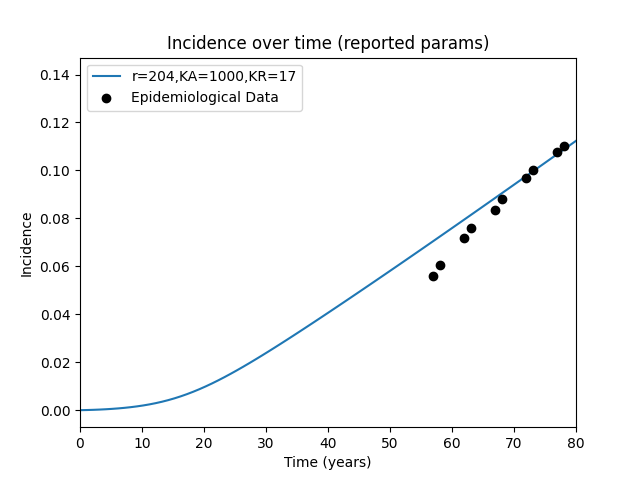
\includegraphics[width=0.65\linewidth]{figures/IncidenceProbabililty_PaperParams.png}
    \caption{Poor fit results when using best fit parameters reported in Wang et. al paper.}
    \label{fig:paper parameters}
\end{figure}
\FloatBarrier
 
It is important to note that their reported best parameter set contained exclusively values with $K_{A} > K_{R}$, while ours contained exclusively values with $K_{R} > K_{A}$, as such, we were unable to corroborate their figure 3c, where best fit parameters are reported to correspond with an APC first biological mechanism. 